%!TEX TS-program = xelatex
%!TEX encoding = UTF-8 Unicode


En el siguiente punto se pueden observar las curvas de modularidad \textbf{(Q)} y número de comunidades \textbf{(NC)} por cada sujeto y para cada estadio del sueño, en lugar de utilizar las matrices promedio como en el punto anterior.

En primer lugar, se aplicó el metodo de Louvain y se obtuvieron los coeficientes de modularidad y el número de comunidades, posteriormente se realizan las comparaciones del estado W contra los estados del sueño N1, N2 y N3 con un t-test, donde analizando los resultados se observó la necesidad de realizar corrección por comparaciones multiples debido a la alta probabilidad de ocurrencia de falsos positivos.

Posteriormente, para realizar la corrección por comparaciones multiples, se realizó un test de ANOVA mixto para los individuos y cada etapa del sueño. Los p valores de las densidades se calcularon con un test de Tukey para controlar la comparación de todos los grupos y se ajustaron siguiendo el método Benjamini-Hochberg.

\begin{figure}[H]
    \centering
    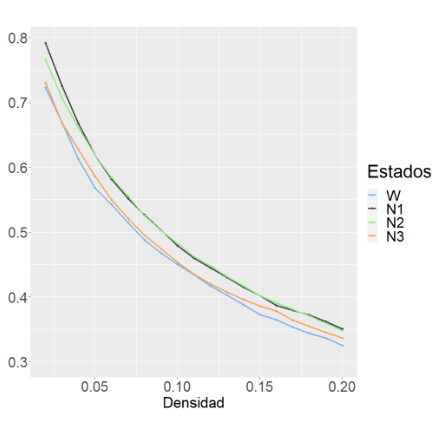
\includegraphics[width = 5in]{img/3_1_Modularidad.jpg}
    \caption{Modularidad}
    \label{fig:3_1_Modularidad}
\end{figure}

En el gráfico de modularidad, donde se comparan los estadíos N1, N2 y N3 contra el estadío W, se puede observar que W y N3 presentan una modularidad similar, sin embargo, los estadíos N1 y N2 presentan valores similares entre sí y una modularidad claramente mayor a W.

\begin{figure}[H]
    \centering
    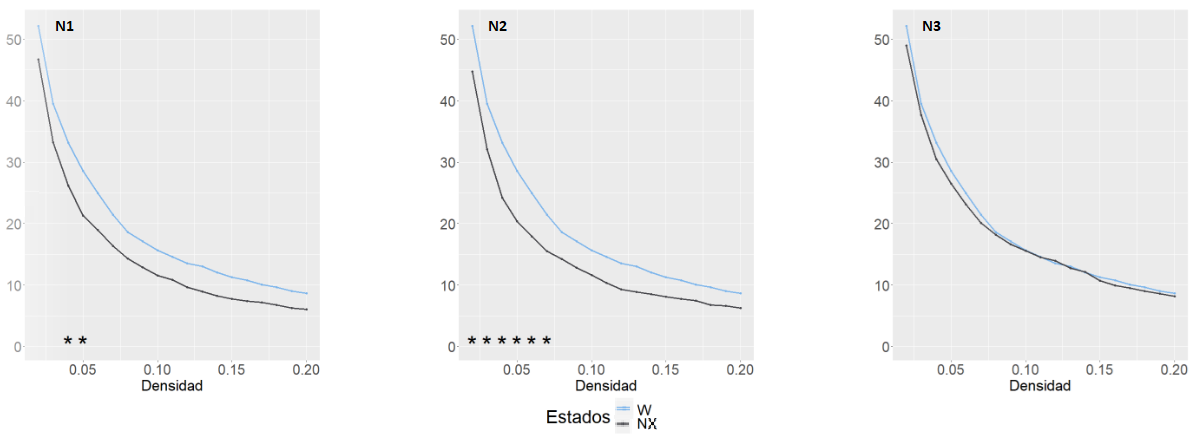
\includegraphics[width=\textwidth]{img/3_2_N_comunidades.jpg}
    \caption{Número de Comunidades}
    \label{fig:3_2_N_comunidades}
\end{figure}


En cuanto al número de comunidades, se repite un análisis similar al anterior, pero se grafica la comparación de cada estadío N1, N2 y N3 con W en gráficos distintos para observar los valores de densidad donde hay resultados significativos (identificados con asteriscos en la parte inferior del gráfico). Para cada estadío, se observa un comportamiento similar al visto en la modularidad, ya que N1 y N2 también presentan un número de comunidades superior a W y con respecto al estadío N3 este presenta valores muy similares a W.
